\documentclass{article}
\usepackage[polish]{babel}
\usepackage[a4paper, margin=2cm]{geometry}
\usepackage{graphicx}
\usepackage{polski}
\usepackage[utf8]{inputenc}
\usepackage{lettrine}
\usepackage{xcolor}
\usepackage[nodayofweek]{datetime}
\renewcommand{\familydefault}{\sfdefault}

\usepackage[autocite=superscript]{biblatex}
\addbibresource{bibliography.bib}

\title{Historia boulderingu i jego pięć znaczących postaci}
\author{Marcin Młynarczyk}
\newdate{date}{11}{6}{2020}
\date{\displaydate{date}}
\definecolor{blue}{cmyk}{.6,.28,0,.04}

\usepackage{sectsty}
\chapterfont{\color{blue}}
\sectionfont{\color{blue}}
\subsectionfont{\color{blue}}

\addto\captionspolish{
  \renewcommand{\contentsname}%
    {\color{blue}Spis treści}%
}

\begin{document}

\maketitle
\tableofcontents

\bigskip

\begin{figure}[!htbp]
	\begin{center}
		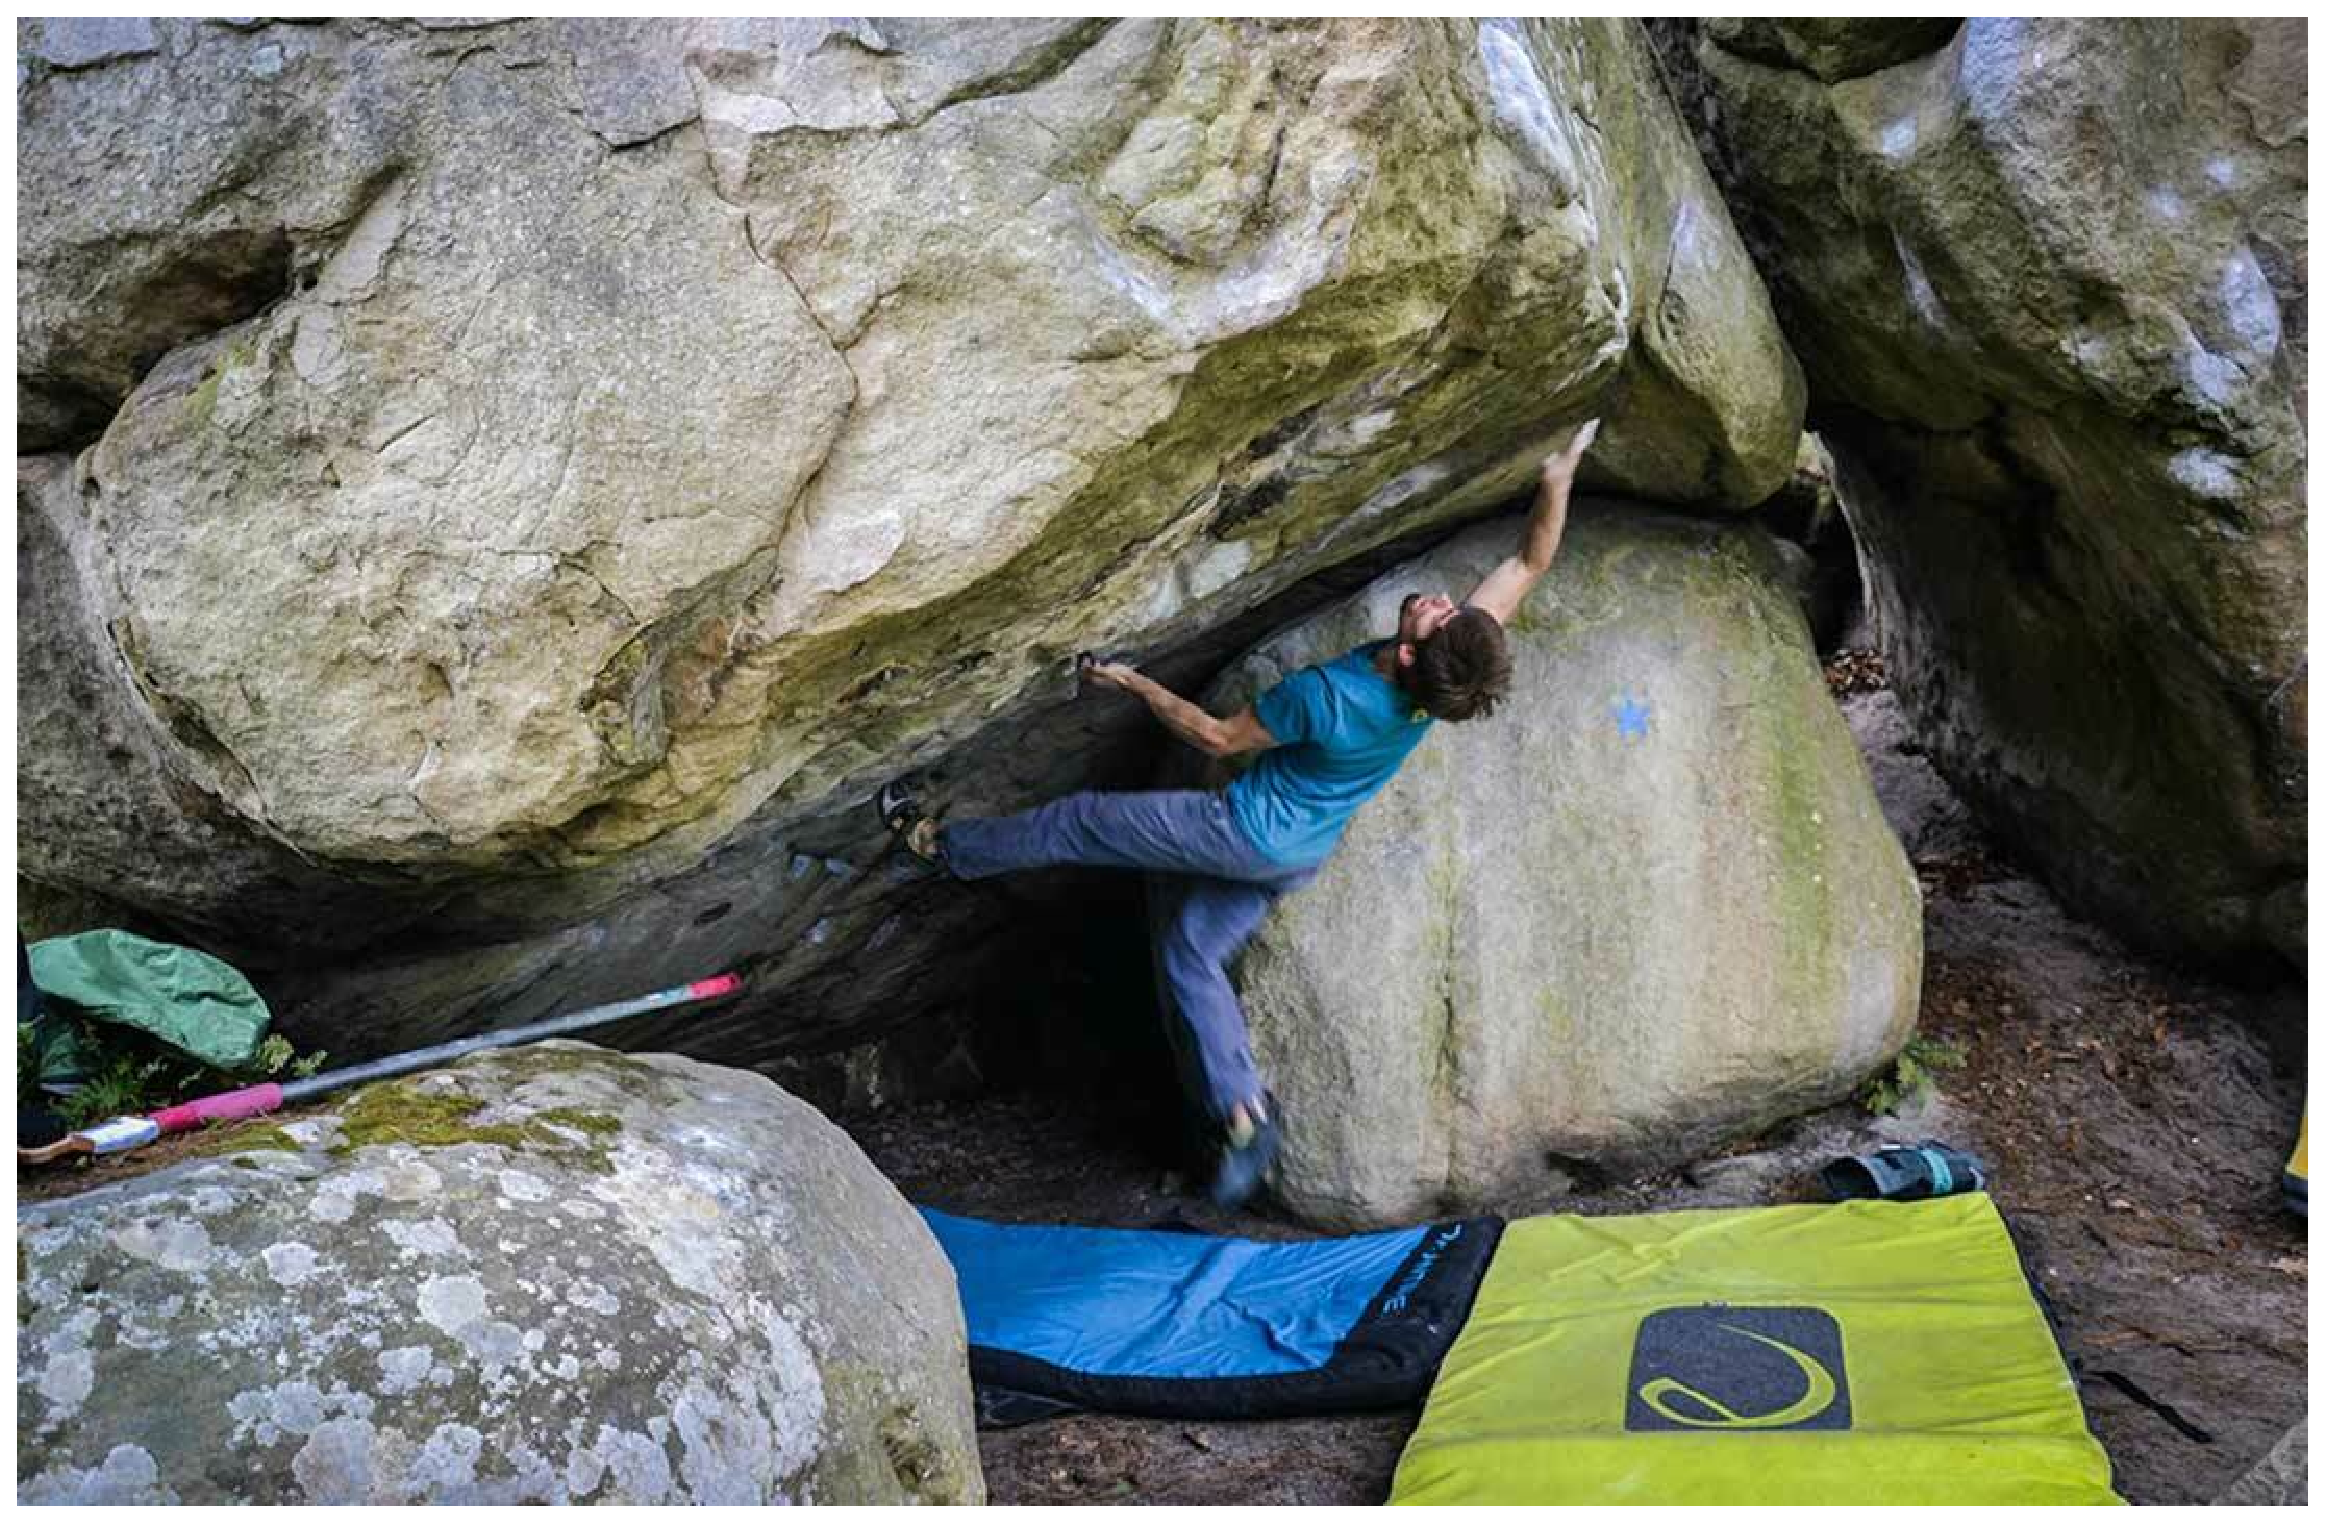
\includegraphics[width=\linewidth]{images/intro.eps}
	\end{center}
	\caption{Roman Batsenko na Gourmandise Raccourci 8A+, Fontainebleau, Francja (fot. Karolina Stawoska) \cite{8a}}
\end{figure}

\section{Wstęp}
\lettrine[lines=2]{B}{ouldering} staje się coraz popularniejszą formą aktywności fizycznej. Owy termin, w swojej angielskiej postaci, dość mocno zakorzenił się w polskim żargonie wspinaczkowym. Pojęcie \textit{bouldering} pochodzi z języka angielskiego, w którym oznacza \textit{głaz}. Zatem uprawianie boulderingu to w dosłownym tłumaczeniu "głazowanie", czyli wspinanie się na głazy. W języku polskim można się również spotkać z lekko spolszczoną wersją tego terminu - \textit{baldering}. W dużym uproszczeniu, i trochę żartobliwie, bouldering można zdefiniować jako "wchodzenie na kamyki od trudnej strony". W odróżnieniu od wspinaczki z liną, asekurację najczęściej stanowią tutaj materace rozłożone w potencjalnej strefie upadku. Z tego również powodu, jako obiekt wspinania obiera się tutaj z reguły wolnostojące głazy poniżej 6 m wysokości. Niemniej jednak, można spotkać od tej reguły wyjątki, np. boulder o nazwie \textit{Ambrosia} w Bishop, Colorado w USA posiada ponad 16 m wysokości \cite{ambrosia}.

\begin{figure}[!htbp]
	\begin{center}
		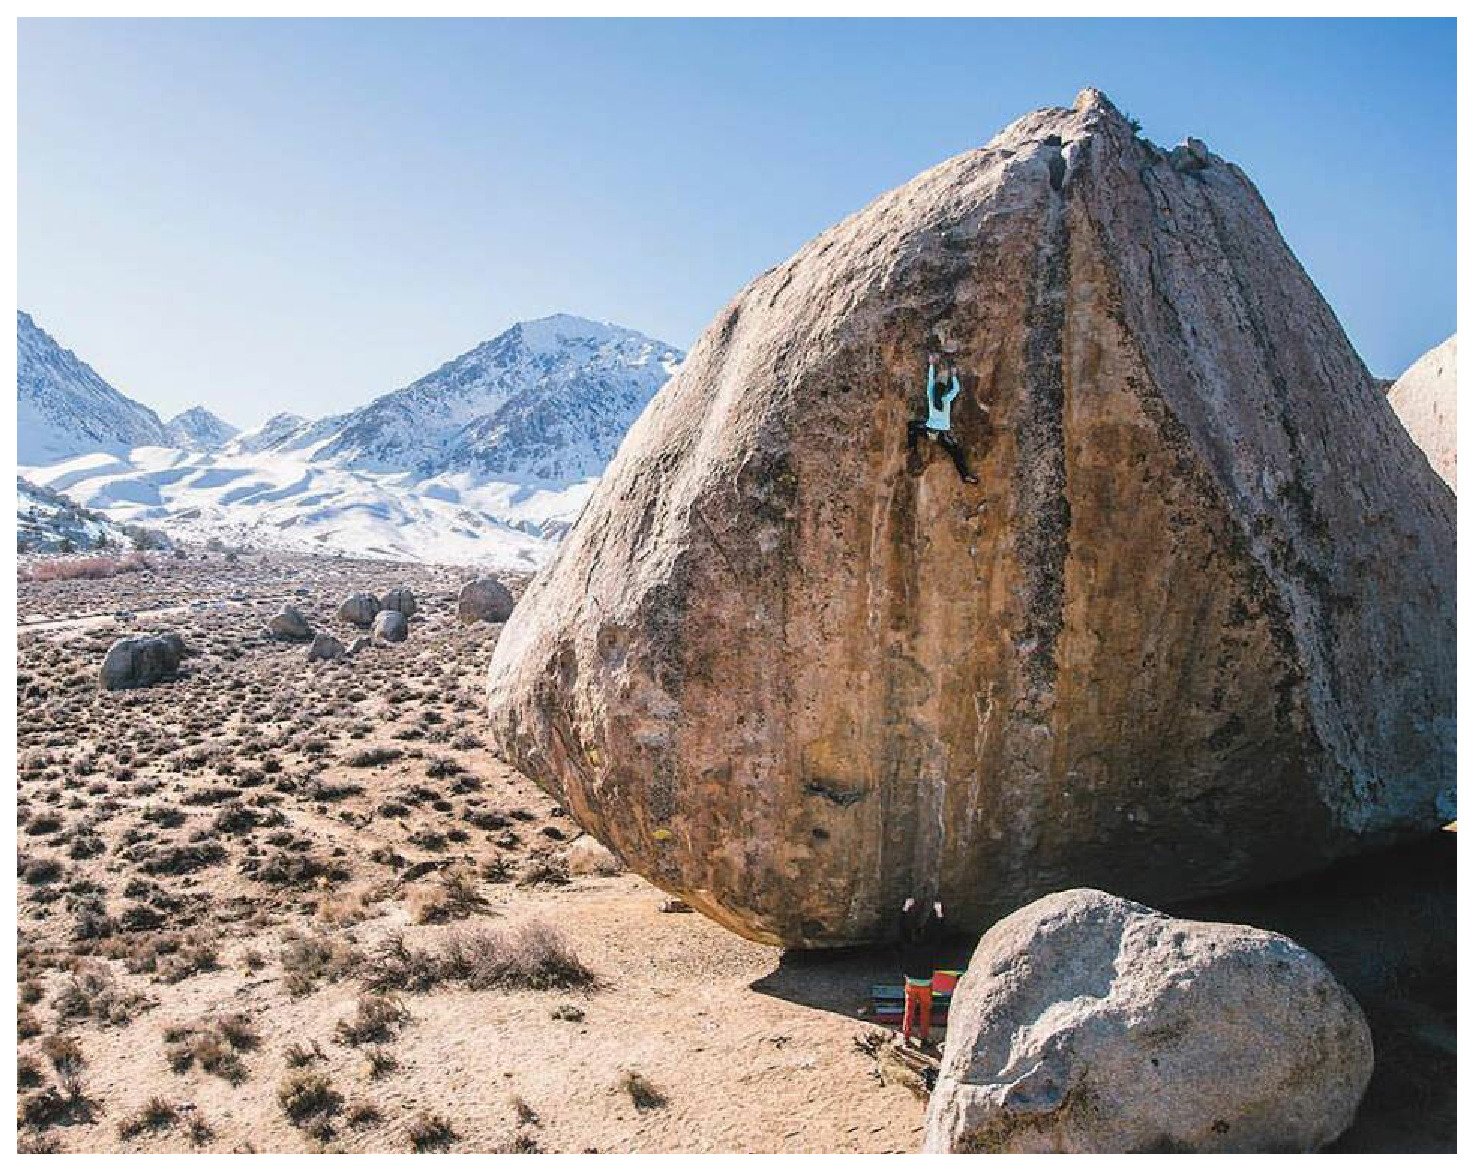
\includegraphics[width=\linewidth]{images/nina-williams-abrosia.eps}
	\end{center}
	\caption{Nina Williams i słynny highball “Ambrosia” (fot. Nayton Rosales) \cite{nina}}
\end{figure}

\section{Historia}
\lettrine[lines=2]{S}{kupię} się na przedstawieniu światowej historii rozwoju omawianego w tej pracy sportu, jako że w dostępnych źródłach bardzo ciężko doszukać się informacji na temat polskiej historii boulderingu. Postaram się przytoczyć okoliczności powstania boulderingu, a następnie przejdę do przedstawienia jego obecnej sytuacji. Wspaniałym źródłem wiedzy o historii boulderingu okazały się materiały \cite{gill-history} napisane przez ojca współczesnego boulderingu - Johna Gill'a - o którym więcej napiszę w sekcji \ref{jg}. W tej pracy, nie jestem w stanie w tak dokładny i ciekawy sposób przekazać dostępnej tam wiedzy, dlatego zaciekawionego czytelnika zachęcam do zapoznania się z owymi materiałami - szczególnie interesującymi są liczne fotografie z przełomu XIX i XX wieku, ukazujące wspinaczy uprawiających czynności jak najbardziej przypominające bouldering (Rysunek \ref{benson}).

\begin{figure}[!htbp]
	\begin{center}
		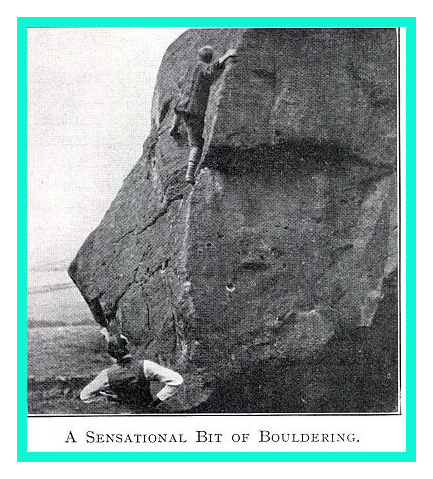
\includegraphics[width=\linewidth]{images/old1.eps}
	\end{center}
	\caption{British Mountaineering, 1909 (fot. Claude E. Benson) \cite{gill-history}}
	\label{benson}
\end{figure}

\subsection{Początki}
Istnieją przypuszczenia, że początki nieudokumentowanego boulderingu sięgają drugiej połowy XIX wieku. Zaczynał wtedy rozkwitać alpinizm i gdy nie dopisywała pogoda, wspinacze mieli ćwiczyć na owych małych głazach jako przygotowanie do późniejszych ekspedycji. Mogliśmy takie praktykie obserwować w m.im. \textit{Fontainebleau} we Francji, czy \textit{Lake District} w Wielkiej Brytanii. Niemniej jednak, takie podejście wspinaczy ukazywało bouldering jako środek do osiągnięcia "wyższych celi" i nie widziało w jego istocie sportu w pełnej okazałości. Ktoś mógłby rozsądnie i dociekliwie zatem zapytać, a z kiedy mamy pierwsze udokumentowane doniesienia o bardziej poważnym podejściu do rozważanej tutaj formy wspinaczki?

Na arenie międzynarodowej, to wspinacz Oscar Eckenstein, pochodzący z Wielkiej Brytanii, wydaje się być prekursorem boulderingu pokazującego oddanie tej dyscyplinie, zbliżone do tej które możemy obserwować w dzisiejszych czasach. Eckenstein żył na przełomie XIX i XX wieku i wspinał się m.in. w rejonie \textit{Lake District}. Aleister Crowley miał rzekomo mówić, że Eckenstein był w stanie pokonać problem na \textit{Y-Boulder} w \textit{Lake District}, którego inni wybitni wspinacze tamtego okresu nie byli w stanie przejść. Zdaniem Johna Gill'a Eckenstein mógłbyć pierwszym prawdziwym mistrzem tego sportu - był wspinaczem, który nie tylko poszerzał standardy trudności, ale również w dość znaczący sposób przyczyniał się do ewolucji filozofii i praktykowania boulderingu.

\subsection{Obecnie}

\section{Znaczące postaci}
\lettrine[lines=2]{W}{} tej sekcji postaram się przedstawić sylwetki znaczących postaci ze względu na historię rozwoju boulderingu - John Gill, John Sherman i Fred Nicole, oraz sylwetki wspinaczy, którzy obecnie posiadają na swoim koncie najtrudniejsze trasy - wśród mężczyzn Nalle Hukkataival i wśród kobiet Ashima Shiraishi. 

\subsection{John Gill}
\label{jg}
\subsection{John Sherman}
\subsection{Fred Nicole}
\subsection{Ashima Shiraishi}
\subsection{Nalle Hukkataival}

\nocite{*}
\printbibliography

\end{document}
